\chapter{Poniendo en marcha \appname}

\label{ref:poniendoenmarcha}\subsection[El asistente de acceso]{El
asistente de acceso}

\begin{center}
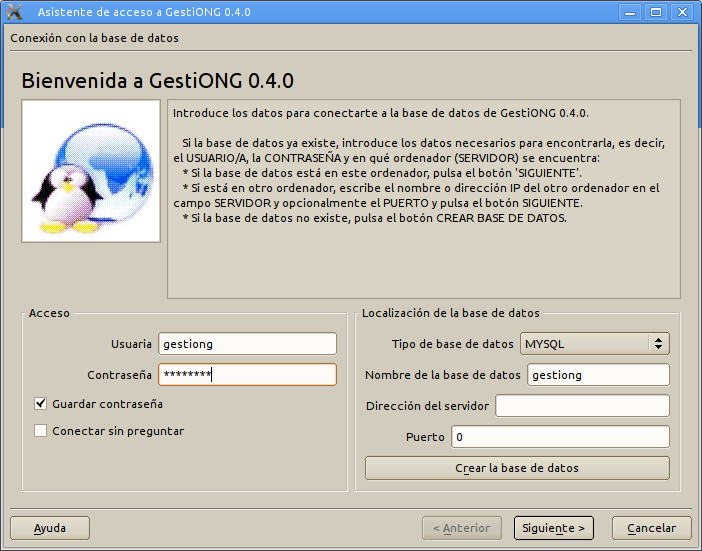
\includegraphics[width=12cm]{bienvenidaagestiong.png}
\captionof{figure}{Asistente de acceso a \appname}
\label{seq:refIllustration3}
\end{center}

Cada vez que ejecutas \appname en tu ordenador, aparece el
{\textquotedblleft}\textbf{\textit{Asistente de acceso a
\appname}}\textbf{{\textquotedblright}} para controlar el acceso a la
base de datos de vuestra asociación. Si la base de datos ya existe, tienes que indicar 
su nombre (\textstyleGUIELEMENT{Nombre de la base de datos}), en qué ordenador
(\textstyleGUIELEMENT{Dirección del servidor} y \textstyleGUIELEMENT{Puerto}) se
encuentra, el nombre de una \textstyleGUIELEMENT{Usuaria} autorizada y
su \textstyleGUIELEMENT{Contraseña} y después pulsar el botón
\textstyleGUIELEMENT{Siguiente (Next)}. 

Sin embargo, la primera vez que ejecutas \appname en tu
asociación, tienes que crear la base de datos. Para ello, necesitas
saber la \textstyleGUIELEMENT{Contraseña de la superusuaria} del
servidor de la base de datos. Los escenarios más frecuentes con los
que te puedes encontrar a la hora de crear la base de datos son, como
has visto en el apartado \textit{Instalando el servidor de la
base de datos}:

\liststyleLv
\begin{enumerate}
\item Si solamente tenéis un ordenador en vuestra asociación,
habrás instalado tanto la base de datos como \appname en el mismo
ordenador, que actuará como servidor:
\end{enumerate}

\textstyleGUIELEMENTREDUCED{NOMBRE DE LA BASE DE DATOS}: gestiong

\textstyleGUIELEMENTREDUCED{DIRECCIÓN DEL SERVIDOR}: (vacío)

\textstyleGUIELEMENTREDUCED{PUERTO}: 0

\textstyleGUIELEMENTREDUCED{NOMBRE DE LA UPERUSUARIA}: root

\textstyleGUIELEMENTREDUCED{CONTRASEÑA DE LA SUPERUSUARIA}: (la que
hayas puesto al servidor MySQL al instalarlo o vacía por defecto)

\liststyleLv
\setcounter{saveenum}{\value{enumi}}
\begin{enumerate}
\setcounter{enumi}{\value{saveenum}}
\item Si tenéis varios ordenadores conectados en red, habrás
instalado la base de datos en uno de ellos, que asumirá el papel de
servidor y podréis instalar \appname en el resto de ordenadores:
\end{enumerate}

\textstyleGUIELEMENTREDUCED{NOMBRE DE LA BASE DE DATOS}: gestiong

\textstyleGUIELEMENTREDUCED{DIRECCIÓN DEL SERVIDOR}: (la dirección
IP del servidor de la base de datos, algo como 192.168.1.120)

\textstyleGUIELEMENTREDUCED{PUERTO}: 0

\textstyleGUIELEMENTREDUCED{NOMBRE DE LA SUPERUSUARIA}: root 

\textstyleGUIELEMENTREDUCED{CONTRASEÑA DE LA SUPERUSUARIA}: (la que
hayas puesto al servidor MySQL al instalarlo o vacía por defecto)

\liststyleLv
\setcounter{saveenum}{\value{enumi}}
\begin{enumerate}
\setcounter{enumi}{\value{saveenum}}
\item También podéis tener la base de datos fuera de la oficina, por
ejemplo, en la sede central de la organización o si habéis
contratado el servicio de base de datos con una empresa externa. En ese
caso, la central o la empresa proveedora os facilitará la
información necesaria para crear la base de datos:
\end{enumerate}

\textstyleGUIELEMENTREDUCED{NOMBRE DE LA BASE DE DATOS}: (proporcionada
por tu proveedora)

\textstyleGUIELEMENTREDUCED{DIRECCIÓN DEL SERVIDOR}: (proporcionado
por tu proveedora, algo como mysql.midominio.org u 84.123.12.34)

\textstyleGUIELEMENTREDUCED{PUERTO}: 0

\textstyleGUIELEMENTREDUCED{NOMBRE DE LA UPERUSUARIA}: (proporcionada
por tu proveedora)

\textstyleGUIELEMENTREDUCED{CONTRASEÑA DE LA SUPERUSUARIA}:
(proporcionada por tu proveedora)

\smallskip

Al mismo tiempo que se crea la base de datos de la asociación, se
creará también una \textstyleGUIELEMENT{Usuaria} con su
correspondiente \textstyleGUIELEMENT{Contraseña} para accesos
posteriores ({\textquotesingle}\textit{gestiong{\textquotesingle}} en
el ejemplo de la \textit{\figurename~\ref{seq:refIllustration3}}). Es
posible añadir más usuarias posteriormente, cada una con un nivel
de acceso adecuado a su rol en la asociación. \ 

\subsection[Creando la base de datos]{Creando la base de datos}
Con todos estos datos a mano, puedes ahora comenzar el proceso de
creación de la base de datos utilizando el
{\textquotedblleft}\textbf{\textit{Asistente de acceso a
\appname}}\textbf{{\textquotedblright}}
(\textit{\figurename~\ref{seq:refIllustration3}}). En importante leer
con atención las instrucciones que aparecen en esta ventana y sobre
todo, la información que aparezca en caso de ocurrir algún error.
En el recuadro \textstyleGUIELEMENT{Acceso a \appname} introduce el
nombre de la \textstyleGUIELEMENT{Usuaria} (y la
\textstyleGUIELEMENT{Contraseña}) con la que usarás habitualmente
el programa, en este ejemplo,
{\textquotesingle}\textit{gestiong}{\textquotesingle}. Completa los
datos con un \textit{1} en el \textstyleGUIELEMENT{N{\textordmasculine}
de asociación} y el \textstyleGUIELEMENT{Ejercicio} actual.

En el recuadro \textstyleGUIELEMENT{Localización de la base de datos},
rellena los datos según el escenario de instalación que hayas
elegido de los tres que has visto más arriba. En el ejemplo de la
\textit{\figurename~\ref{seq:refIllustration3}}, la base de datos se
encontraría en tu propio ordenador. 


\bigskip

Ahora pulsa el botón \textstyleGUIELEMENT{Crear la base de datos},
tras lo cual el asistente mostrará esta nueva ventana
(\textit{\figurename~\ref{seq:refIllustration4}}):

\begin{center}
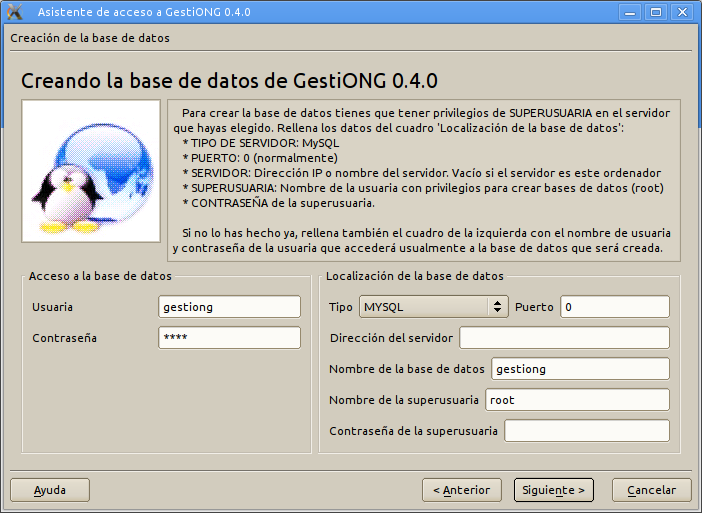
\includegraphics[width=12cm]{creandolabasededatos.png}
\captionof{figure}{Asistente para la creación de la base de datos}
\label{seq:refIllustration4}

\end{center}
En el recuadro \textstyleGUIELEMENT{Localización de la base de datos}
deberás introducir la \textstyleGUIELEMENT{Dirección
del servidor}, el \textstyleGUIELEMENT{Nombre de la superusuaria,} que será casi siempre
{\textquotesingle}\textit{root}{\textquotesingle}, la
\textstyleGUIELEMENT{Contraseña de la superusuaria,} y pulsar el
botón \textstyleGUIELEMENT{Siguiente (Next).} Si todo va bien,
vuestra base de datos se habrá creado correctamente y pasarás a la ventana principal. 


\subsection{La ventana principal}
Ya tienes, por fin, creada la base de datos y la asociación. Ahora
aparece la ventana principal de \appname, el entorno donde trabajarás
con los ficheros y los procesos cotidianos de gestión.
